\documentclass[]{report}
\usepackage{amsmath}
\usepackage[spanish]{babel}
\usepackage[utf8]{inputenc}
\usepackage{amsmath}
\usepackage[spanish]{babel}
\usepackage{graphicx}

\usepackage[top=2cm, bottom=2cm, left=3cm, right=3cm]{geometry}


% Título y detalles del TP
\title{Introducción al Modelado Continuo \\[0.5cm]
	Trabajo Práctico 1 \\[0.5cm]
	Trayectorias de Kepler y Corrección Relativista}

% Sección de integrantes y grupo
\author{
	\textbf{Grupo: 11} \\ [1cm]
	\begin{tabular}{llll}
		\textbf{Apellido} & \textbf{Nombre} & \textbf{Libreta} \\ \hline
		Wilders Azara & Santiago & 350/19  \\
		Peralta & Martín & 428/22 \\
		Vernay & Jerónimo & 313/24 \\
	\end{tabular}
}

%Fecha
\date{\today}

\setlength{\parindent}{0pt}
\setlength{\parskip}{1ex plus .5ex minus .2ex}

\begin{document}
\maketitle
%\begin{abstract}
%\end{abstract}

% --- Desarrollo de los ejercicios ---

\section*{Enunciado}

Una corrección relativista para el problema de dos cuerpos de Kepler, sistema Sol-planeta, puede describirse en coordenadas polares con la ecuación:
$$
\ddot{u}(\theta) + u(\theta) - \frac{1}{\alpha} - \delta u^{2}(\theta) = 0
$$
Donde $u(\theta) = \frac{1}{r(\theta)}$, el Sol se encuentra en el origen, $\alpha$ y $\delta$ son constantes. El término con $\delta$ es la corrección relativista.

\section*{Ejercicio 1}

\subsection*{Consigna.}

Formular el problema como un sistema de orden uno de la forma $\dot{y} = f (\theta, y)$. Observar que la variable independiente no es el tiempo sino ángulos en polares.

\subsection*{Resolución.}

La ecuación original está dada por

$$\ddot{u}(\theta) + u(\theta) - \frac{1}{\alpha} - \delta u^2(\theta) = 0$$

Reducción de orden:

\begin{equation*}
	\begin{aligned}
		y_1 &= u \\
		y_2 &= \dot{u} \\
		\dot{y_2} &= \ddot{u}
	\end{aligned}
	\quad \implies \quad 
	\dot{y_2} + y_1 - 1/a - \delta y_1^2 = 0
	\quad \implies \quad
	\begin{aligned}
		\dot{y_1} &= y_2 \\
		\dot{y_2} &= \delta y_1^2 + 1/a - y_1
	\end{aligned}
\end{equation*}

El estado del sistema queda definido por la inversa de la distancia radial ($y_1 = u(\theta)$) y su tasa de cambio respecto al ángulo ($y_2 = \dot{u}(\theta)$). Como el ángulo $\theta$, la variable independiente, no aparece de forma explicita en las ecuaciones, obtenemos un sistema autónomo no lineal de primer orden.

Para justificar analíticamente que $\theta$ actúa como la única variable independiente del sistema, es necesario demostrar cómo se elimina la dependencia del tiempo t en las ecuaciones de movimiento. Este procedimiento se fundamenta en la conservación del momento angular.

En coordenadas polares, el momento angular del planeta respecto al Sol se define como $L = r \times p$, donde $p = mv$ es el momento lineal. La variación temporal de esta magnitud está determinada por el torque neto aplicado sobre el sistema ($\tau = r \times F$), tal que:
$$
\frac{dL}{dt} = \tau
$$

En el modelo de Kepler, la única fuerza que interviene en el movimiento del planeta es la atracción gravitacional. Al tratarse de una fuerza central, su vector $\vec{F}$ actúa sobre la misma línea que une al planeta con el Sol, resultando paralelo al vector de posición radial $\vec{r}$.
Dado que ambos vectores son paralelos, su producto vetorial se anula (y consecuentemente el torque $\tau = 0$), garantizando que el \textbf{momento angular se conserve} en el tiempo.

La magnitud del momento angular se puede expresar mediante la masa $m$ y la componente tangencial de la velocidad del planeta ($v_{\theta} = r \dot{\theta}$):
$$
L = m r v_{\theta} = m r \left(r \dot{\theta}\right) = m r^2 \dot{\theta} = cte
$$

Dado que la masa es invariable, se deduce que:
$$
r^2 \dot{\theta} = cte
$$

Esta relación permite transformar el operador que deriva en función del tiempo ($\frac{d}{dt}$) usando la regla de la cadena:
$$
\frac{d}{dt} = \frac{d\theta}{dt} \frac{d}{d\theta} = \frac{r^2}{r^2} \frac{d\theta}{dt} \frac{d}{d\theta} = \frac{r^2 \dot{\theta}}{r^2} \frac{d}{d\theta} = \frac{cte}{r^2} \frac{d}{d\theta}
$$

Para aplicar este operador nuevo sobre la coordenada radial $r$, primero debemos obtener cómo cambia $r$ con respecto al ángulo $\theta$ (sabiendo que $u = \frac{1}{r}$):
$$
\frac{dr}{d\theta} = \frac{du}{d\theta} \frac{dr}{du} = - \frac{1}{u^2} \frac{du}{d\theta} 
$$

Volviendo al caso de la ecuación diferencial, reemplazamos el operador temporal y la derivada de $r$ obtenida para reescribir la velocidad radial:
$$
\frac{dr}{dt} = \left(\frac{cte}{r^2} \frac{d}{d\theta}\right) r = \frac{cte}{r^2} \frac{dr}{d\theta} = cte \cdot u^2 \left(-\frac{1}{u^2} \frac{du}{d\theta}\right) = - cte \ \frac{du}{d\theta}
$$

De manera análoga, se puede observar que ocurre lo mismo con la aceleración radial $\ddot{r}$: las derivadas temporales se reemplazan por derivadas respecto a $\theta$.

En una ecuación diferencial ordinaria, la variable respecto a la cual se aplican las derivadas es, por definición, la variable independiente.
Así, el tiempo desaparece por completo del modelo y queda demostrado que el estado del sistema depende exclusivamente del ángulo polar $\theta$. 

\newpage

\section*{Ejercicio 2}

\subsection*{Consigna.}

Resolver el problema de Kepler ($\delta= 0$), con condiciones iniciales $r(0) = \frac{\alpha}{1 + \epsilon}$ y $\dot{r}(0) = 0$. Donde $\epsilon$
es la excentricidad de la órbita: $0 \leq \epsilon < 1$ para orbitas cerradas, $\epsilon \geq 1$ para órbitas abiertas. La
condición $\dot{r}(0) = 0$ (velocidad radial cero) significa que medimos los ángulos a partir del perihelio
(punto más cercano al Sol). 

Graficar soluciones con $\alpha = 1$ para distintos valores de $\epsilon$. Observar que pasa cuando $\theta > 2\pi$ (3 o
4 vueltas).

\subsection*{Resolución.}

Nota: el perihelio es el punto de la órbita más cercano al sol, el afelio el más alejado.

Con $\delta = 0$, queda una ecuación diferencial no homogénea:
$$
\ddot{u}(\theta) + u(\theta) = \frac{1}{\alpha}
$$

La resolución numérica se llevó a cabo usando el método \texttt{solve\_ivp} de la librería \texttt{scipy}.
El análisis se divide en el estudio del espacio de fases de las variables de integración ($u$ y $\dot{u}$) y la posterior reconstrucción de las trayectorias.

\textbf{Análisis en el espacio de fases ($u$ vs $\dot{u}$)}

Mediante el dibujo del campo vectorial, se aprecia que todas las trayectorias se estructuran en torno a un punto de equilibrio ubicado en ($u = 1/\alpha$, $\dot{u} = 0$).
Al establecer las condiciones iniciales con velocidad radial nula y posición máxima ($u(0)$) igual a $\frac{1 + \epsilon}{\alpha}$, se fuerza al sistema a iniciar su evolución desde el perihelio.

Aclaración: inicia su evolución desde el perihelio porque la condición inicial es $u$ en su máximo valor, lo que se traduce en el mínimo valor que toma $r$ (porque son inversamente proporcionales), que es la distancia al Sol.

El comportamiento del sistema es claramente influenciado por el valor que toma $\epsilon$:

\begin{itemize}
\item \textbf{Órbitas cerradas ($\epsilon < 1$):} 
Estas órbitas (en el espacio de fases) describen curvas cerradas alrededor del punto de equilibrio. 
Al restringir la integración a $\theta < 1.5\pi$, se evidencia cómo el planeta recorre el ciclo sin llegar a completarlo (véase Figura 1).
La variable $u$ varía de forma continua entre el afelio y el perihelio.

\item \textbf{Órbitas abiertas ($\epsilon \geq 1$):} 
Para valores como $\epsilon = 1.2$, el sistema describe trayectorias hiperbólicas abiertas. 
En el plano de fases, la curva no llega a rodear completamente el punto de equilibrio, el cuerpo termina desligándose del sistema.
\end{itemize}

\textbf{Comportamiento a múltiples vueltas ($\theta > 2\pi$)}
Cuando se extiende el intervalo de integración a 4 vueltas completas ($\theta_{\max} = 8\pi$), se observa que las trayectorias en el espacio de fases se superponen sobre sí mismas (véase Figura 2).
Estas forman una única curva, evidenciando la naturaleza periódica del sistema.

\textbf{Geometría de las órbitas en el plano ($x$,$y$)}

Para trasladar los resultados al espacio físico bidimensional, se aplicó la transformación de coordenadas $r(\theta) = \frac{1}{u(\theta)}$, con proyecciones $x = r \cdot \cos(\theta)$ e $y = r \cdot \sin(\theta)$ (véase Figura 3).

\begin{itemize}
	\item Las curvas generadas con $\epsilon = 0.4$ y $\epsilon = 0.7$ forman elipses, donde el Sol ocupa uno de los focos. A mayor valor de $\epsilon$, el foco se aleja del centro geométrico de la órbita, incrementando el achatamiento de la elipse.
	\item La curva generada con $\epsilon = 1.2$ genera una hipérbola. La trayectoria se aproxima al Sol, alcanza su mínima distancia en el perihelio, y luego se aleja indefinidamente, confirmando el escape del cuerpo.
\end{itemize}

\begin{figure}[htbp]
    \centering
    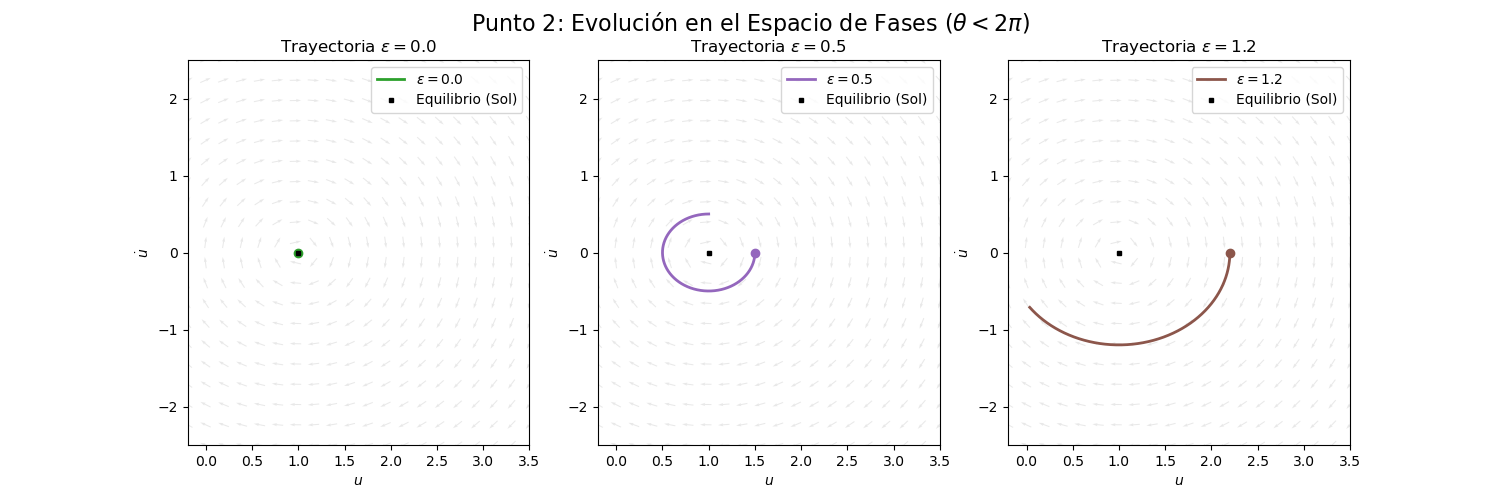
\includegraphics[width=0.7\textwidth]{../Graficos/Evolucion en el espacio de fases. Punto 2.png}
    \caption{Evolución en el espacio de fases ($\theta < 2\pi$).}
    \vspace{0.5cm} % Espacio opcional entre figuras
    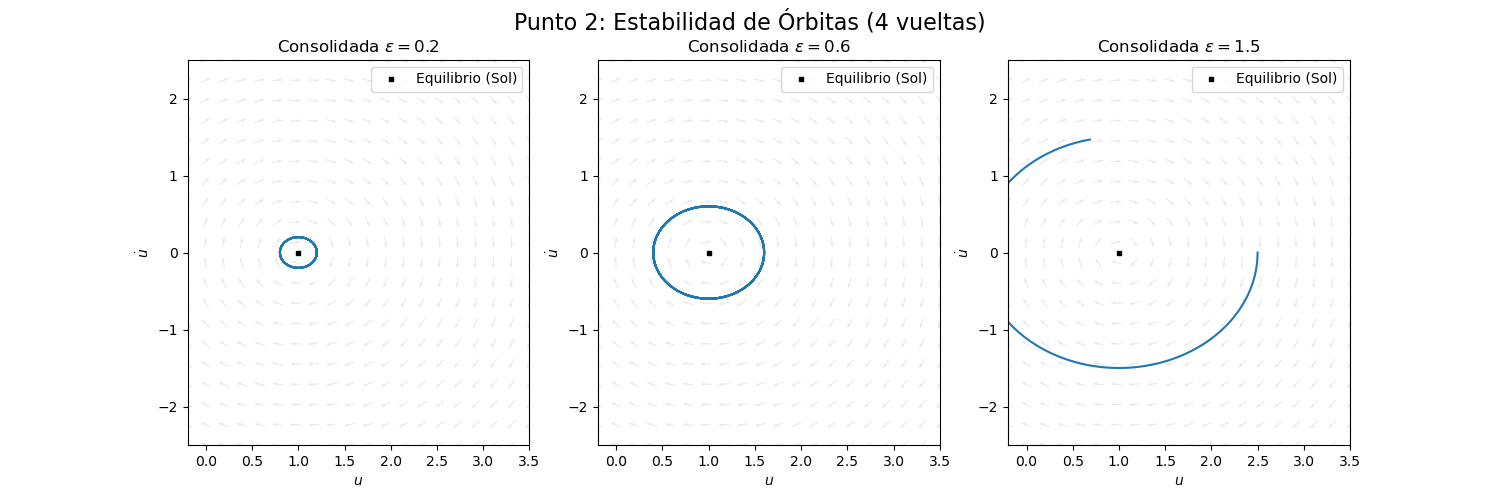
\includegraphics[width=0.7\textwidth]{../Graficos/Punto 2. Estabilidad de las orbitas (4 vueltas).png}
    \caption{Evolución en el espacio de fases para $\theta_{\max} = 8\pi$.}
    \vspace{0.5cm}
    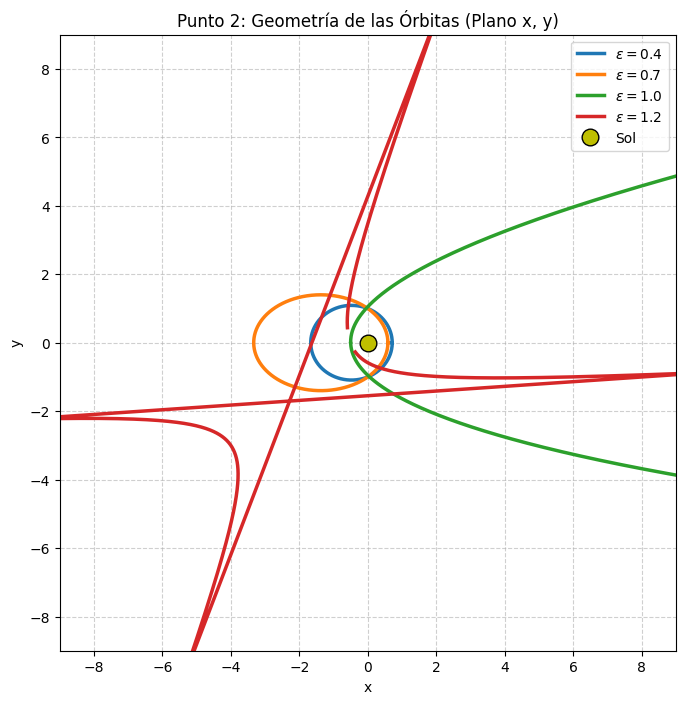
\includegraphics[width=0.5\textwidth]{../Graficos/Punto 2. Geometria de las orbitas en plano cartesiano.png}
    \caption{Geometría de órbitas en el plano cartesiano ($x$, $y$).}
\end{figure}

\newpage
\section*{Ejercicio 3}

\subsection*{Consigna.}

Resolver el problema relativista para $\delta = 0.05$ en las mismas condiciones iniciales del ítem anterior
y comparar.

El efecto se conoce como precesión del perihelio y las mediciones sobre la órbita de Mercurio fueron
utilizadas por Albert Einstein como evidencia experimental de la Teoría General de la Relatividad.

\subsection*{Resolución.}

\textbf{Observaciones del nuevo modelo incorporando la corrección relativista.}

\textbf{Variación del parámetro $\alpha$:}

El valor de $\alpha$ escala directamente las dimensiones de la órbita. Este impacta tanto en el radio del perihelio (punto de distancia radial mínima, $r_{min} = \frac{\alpha}{1+\epsilon}$) como en el radio del afelio (punto de distancia radial máxima, $r_{max} = \frac{\alpha}{1-\epsilon}$). Un aumento en $\alpha$ expande la órbita en su totalidad, incrementando ambos extremos radiales. Por el contrario, una disminución de $\alpha$ reduce los radios y contrae la trayectoria.


\textbf{Variación de la excentricidad ($\epsilon$):}

\textbf{$\epsilon < 1$ (Órbitas cerradas):}

La trayectoria describe un cuerpo de distancia radial acotada con respecto a la estrella central, formando una forma de roseta alrededor de ella. Si disminuimos la excentricidad ($\epsilon \to 0$), cada pétalo de la roseta tiende a circularizarse, el radio del perihelio crece y el del afelio decrece. En cambio, a medida que $\epsilon$ se acerca a $1$, los pétalos se vuelven más estirados, resultando en un decrecimiento del radio del perihelio y un crecimiento del afelio.

\textbf{$\epsilon \ge 1$ (Órbitas abiertas):}\\
Para $\epsilon = 1$, la órbita describe una elipse cerrada. Cuando $\epsilon > 1$, la distancia máxima deja de estar acotada, la trayectoria describe un cuerpo celeste que no se encuentra absorto en la gravedad generada por la estrella central, con forma de hipérbola, alejándose hacia el infinito siguiendo líneas asintóticas.

\begin{figure}[htbp]
	\centering
	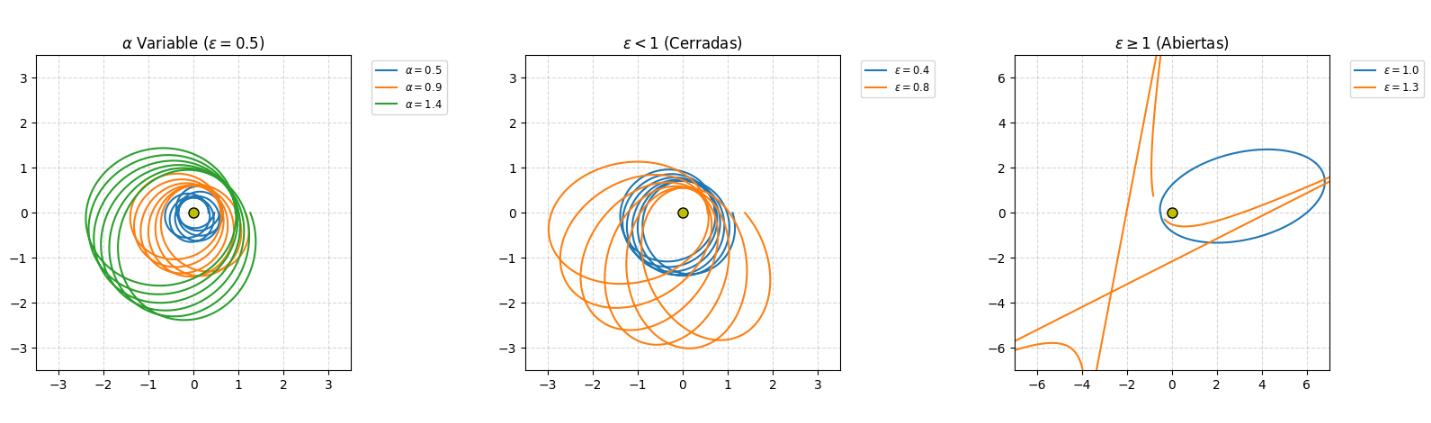
\includegraphics[width=1\textwidth]{../Graficos/Punto 3. Variacion de parametros en coordenadas cartesianas.png}
	\caption{Variación de parámetros en el modelo relativista.}
\end{figure}
\newpage

\textbf{Comparativa entre el modelo clásico de Kepler y la corrección relativista}

Al incorporar el término no lineal de perturbación $\delta > 0$ al sistema (que introduce una dependencia con la inversa del cubo de la distancia), observamos de manera inmediata que las trayectorias ya no definen una elipse perfecta. Es decir, pierden la periodicidad estricta de $2\pi$ en el ángulo orbital. 

Para un valor de $\delta = 0.05$, la trayectoria pasa a describir lo que visualmente se asemeja a una flor, formalmente conocida como órbita de roseta. En términos del perihelio, vemos un desplazamiento progresivo del punto de mínima distancia radial, la trayectoria necesita un ángulo mayor a $2\pi$ para volver a este punto crítico, perdiendo así su capacidad de definir una órbita espacialmente cerrada en un solo ciclo. Este fenómeno astronómico es el que se conoce como la "precesión del perihelio", el cual fue correctamente descrito para la órbita de Mercurio gracias a la corrección relativista.

Al observar el espacio de fases ($u$ frente a $\dot{u}$), el sistema sigue manteniendo un comportamiento periódico en sus variables de estado, el planeta sigue oscilando de forma estable entre un máximo y un mínimo de distancia, por lo que seguimos viendo una elipse. Sin embargo, en el caso relativista, esta elipse se percibe un poco más pequeña respecto a la clásica. Esto ocurre porque el término de perturbación $\delta u^2$ introduce una atracción adicional en el sistema. Otra consecuencia visible es que en el modelo de Kepler, para $\epsilon = 1$ obtenemos una trayectoria parabólica de escape, sin embargo, aquí el sistema no cuenta con la energía suficiente para vencer la atracción extra, resultando en una órbita ligada.

\begin{figure}[htbp]
	\centering
	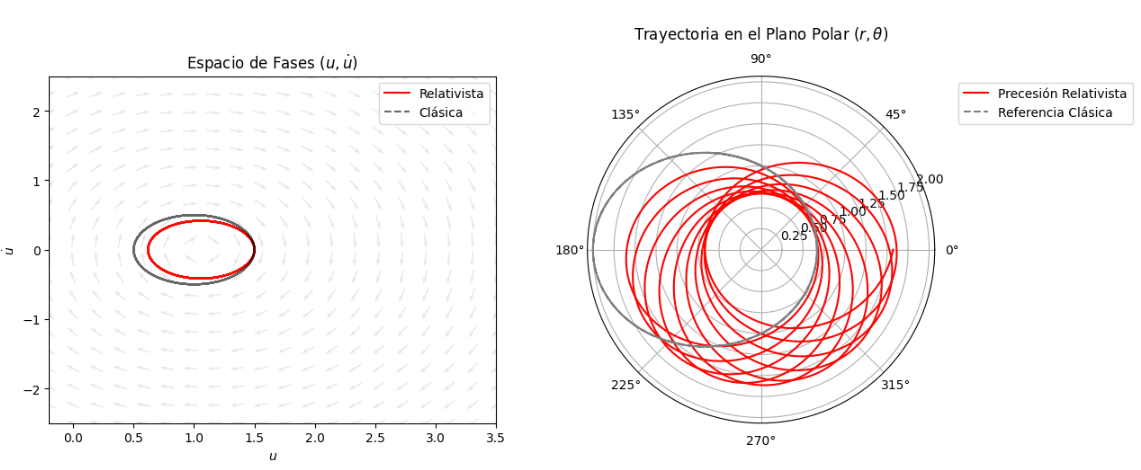
\includegraphics[width=0.9\textwidth]{../Graficos/Punto 3. Precesion del Perihelio.png}
	\caption{Comparación entre el modelo clásico (Kepler) y el modelo relativista.}
\end{figure}


\end{document}